\section{Экспериментальные данные}

Резонанс ЛПП димеров исследовался с помощью микроспектроскопии пропускания. Схема экспериментальной установки показана на рис.~\ref{img:expsetup}. Она состояла из источника света --- галогенной лампочки мощностью 60Вт и спектральным диапазоном $ \lambda =  $ 400 -- 1400 нм, собирающей линзы с фокусным расстоянием 50 мм для формирования параллельного пучка, призмы Глана-Тейлора для преобразования излучения в линейно поляризованное, апертурной диафрагмы и системы из двух объективов с числовой апертурой 0.13 и 10 кратным увеличением. Минимальный диаметр перетяжки составлял 50 мкм. Далее свет собирался в оптоволокно и анализировался спектрометром S100 компании Solar LS.
\begin{figure}
\center{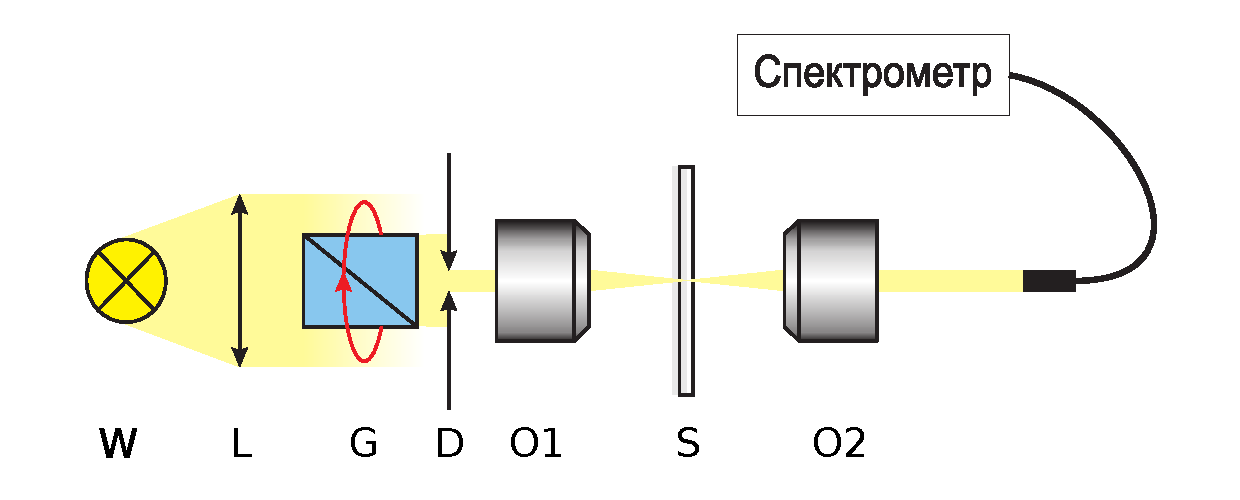
\includegraphics[width=12cm]{img/microspectroscopy/exp_setup.pdf}}
\caption{Схема экспериментальной установки. W --- источник света, L --- собирающая линза для формирования параллельного пучка света, G --- призма Глана-Тейлора для преобразования излучения в линейно поляризованное, D --- апертурная диафрагма, O1, O2 --- система из двух объективов, S --- исследуемый образец. }
\label{img:expsetup}
\end{figure}
Спектры пропускания получались следующим образом: снимался спектр пропускания образца $ S_{sig} $, потом на расстоянии $ \approx 100 $ мкм от ансамбля димеров снимался спектр пропускания подложки $ S_{back} $. Конечный спектр пропускания $ S $ образцов определялся следующим образом:
\begin{equation}
S = \frac{S_{sig}}{S_{back}}.
\end{equation}
Для избавления от шумов каждая точка спектра сглаживалась по 15ти соседним с гауссовым весом. При определении положения резонанса выбиралась точка с минимальным коэффициентом пропускания, а также 20 соседних точек, и полученная кривая аппроксимировалась параболой $ y(x) = y_0 + (x - x_0)^2 $, где точка $ x_0 $ являлась положением резонанса ЛПП. Обработка данных производилась с помощью скрипта, написанного на языке программирования PYTHON.

% Возможно часть, что ниже надо переделать
% BEGIN
% Начало отредактированной части
При получении спектров пропускания было выбрано два направления поляризации: параллельное наностержням и перпендикулярное им. При падении света с поляризацией, перпендикулярной наностержням, наблюдался небольшой сдвиг резонанса ЛПП в красную область спектра при уменьшении расстояния между наностержнями. При падени света с поляризацией, параллельной наностержням, наблюдался сдвиг резонанса ЛПП в синюю область в случае наностержней с длиной $ a = $ 300, 400, 500 нм. В случае наностержней с длиной $ a = $ 100, 150, 200 нм резонанс ЛПП ведет себя неадекватно. Поведение резонанса ЛПП для димеров с длиной наностержней $ a = $ 100 нм и $ a = $ 400 нм и различным расстоянием $ d $ между наностержнями показано на рис.~\ref{img:general}e и рис.~\ref{img:general}f.
\begin{figure}[!h]
\center{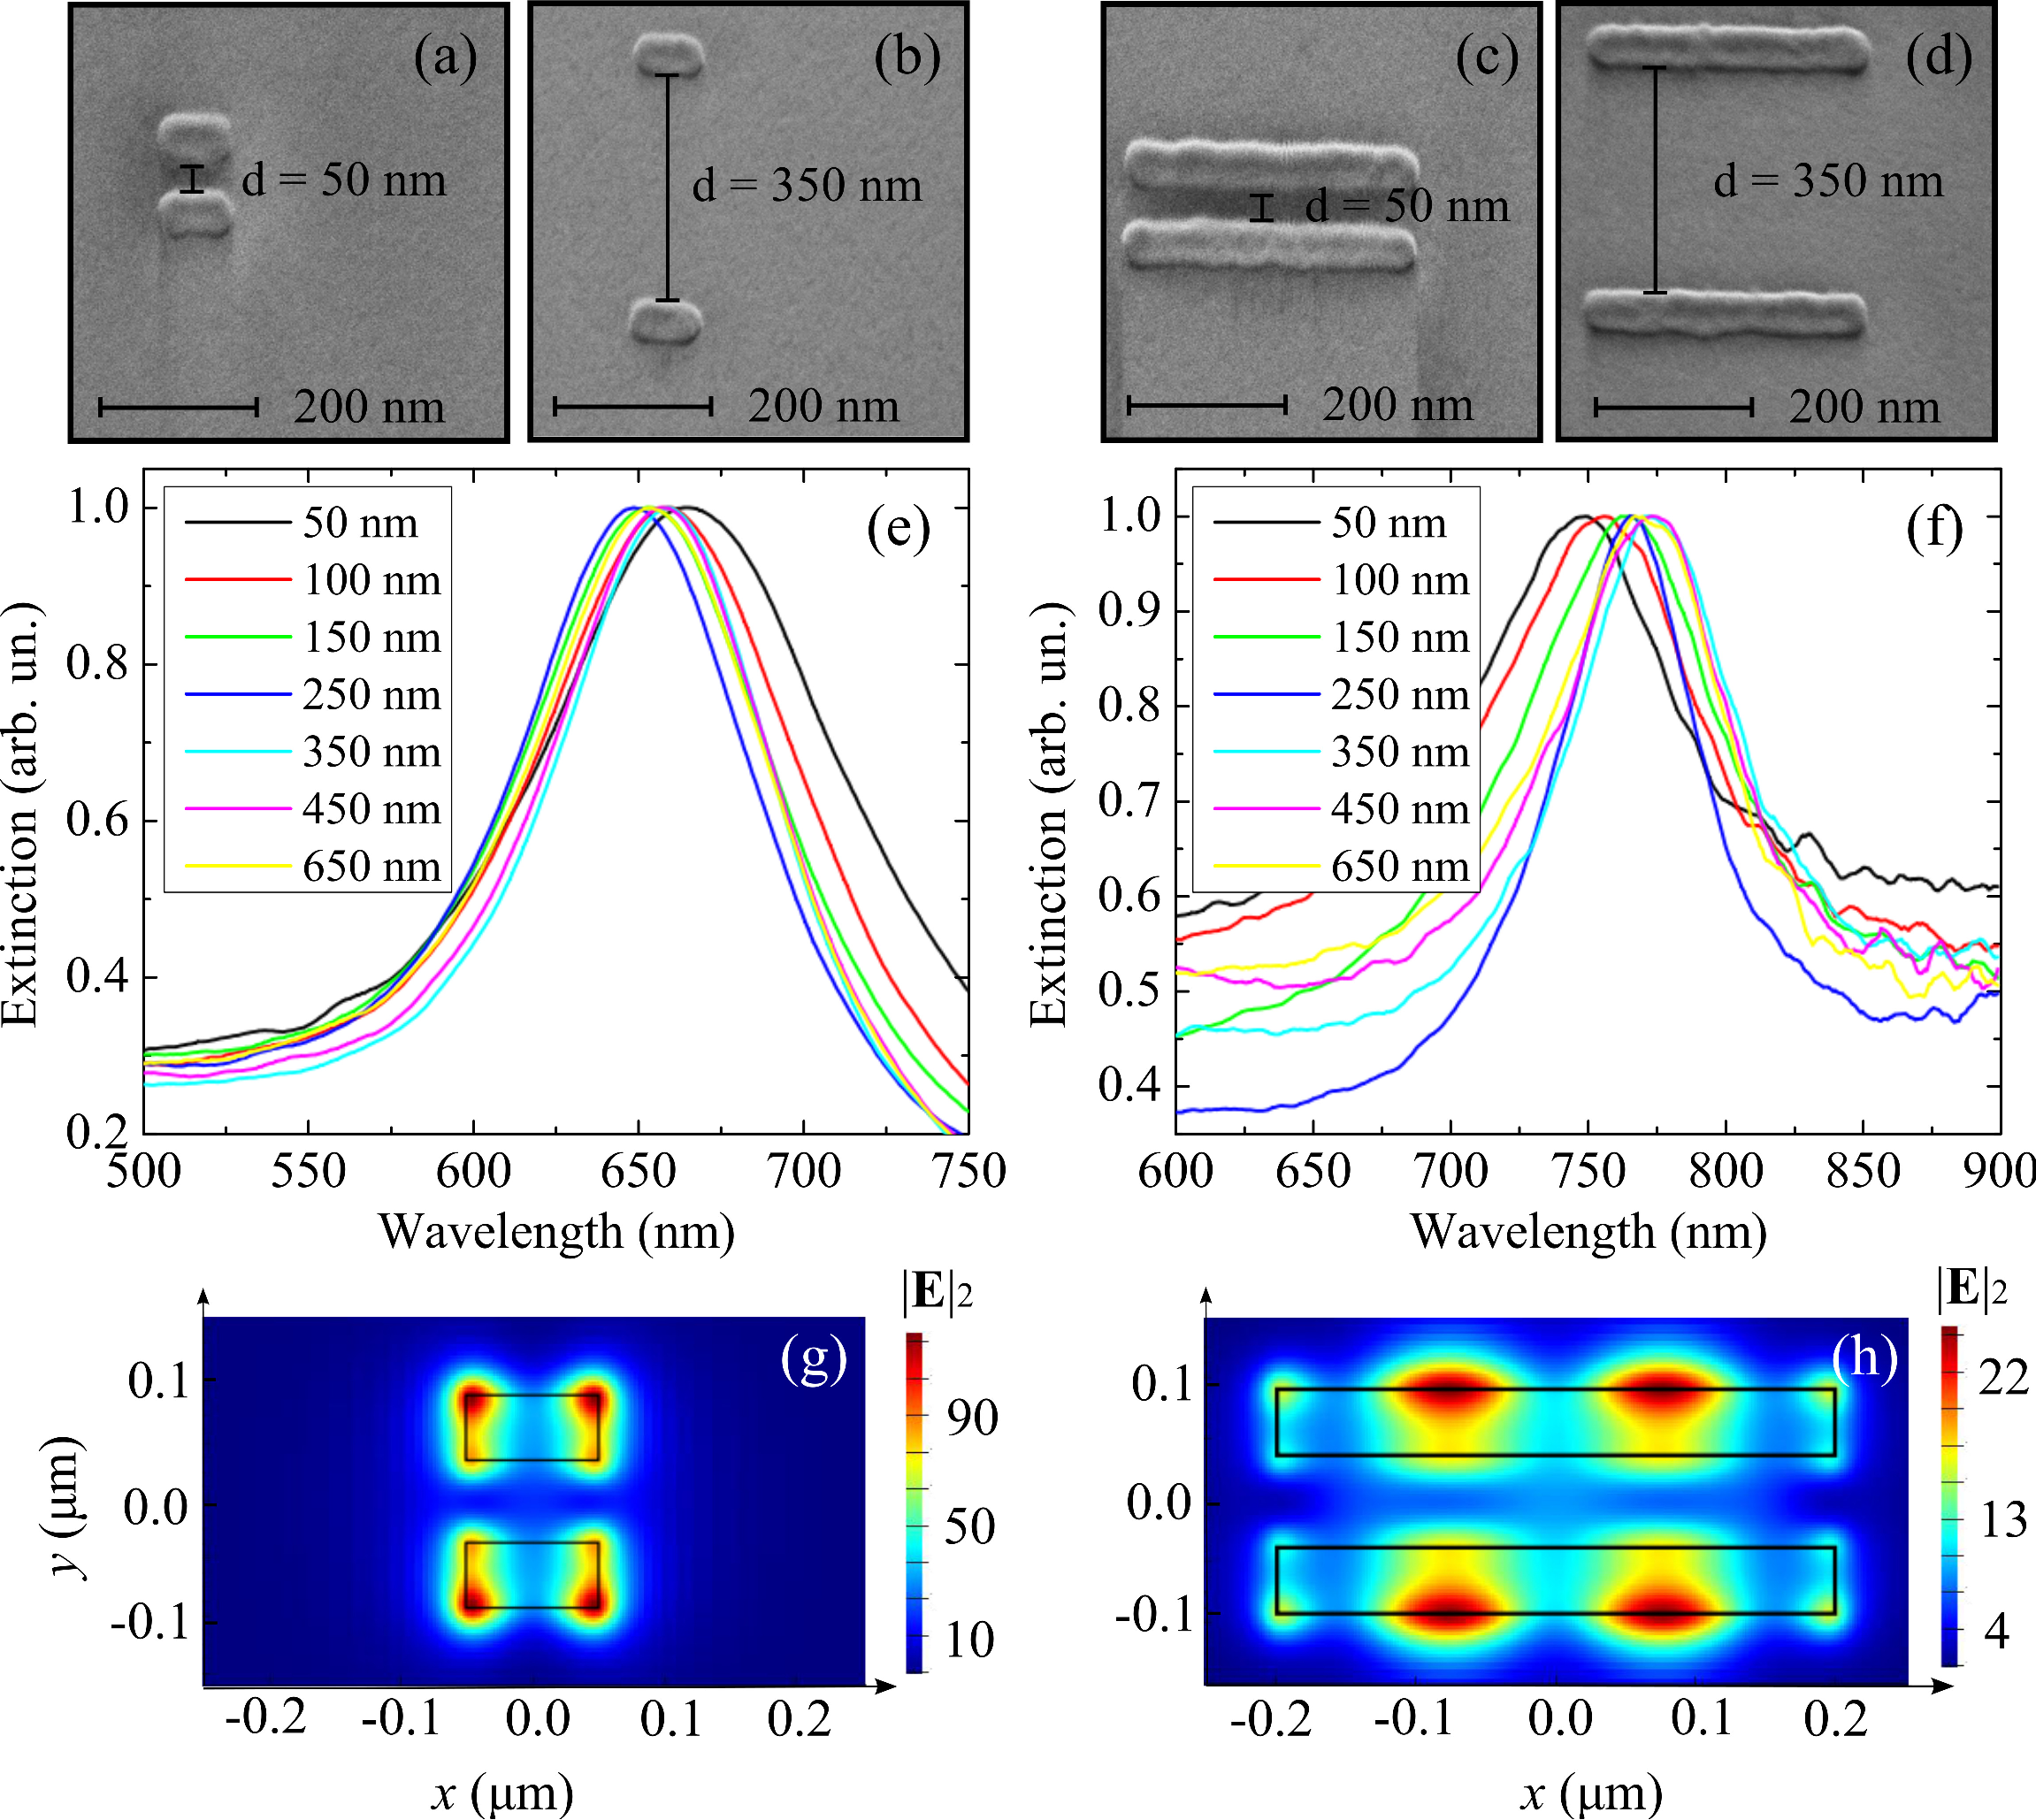
\includegraphics[width=12cm]{img/microspectroscopy/general.pdf}}
\caption{(a-d) Изображения с расторового электронного микроскопа $ \pi $-димеров золотых наностержней с длиной наностержней $ a = $ 100 нм (a-b) или $ a = $ 400 нм (c-d) и расстоянием между наностержнями $ d = $ 50 нм (a,c) или $ d = $ 350 нм (b, d). (e-f) Нормированный экспериментальный спектр экстинкции димеров с длиной наностержней $ a = $ 100 нм (e) и $ a = $ 400 нм (f), относящиеся к резонансу первого и второго порядка, соответственно. (g-h) Численно рассчитанная плотность ЭМ поля вблизи образца в случае резонанса первого или второго порядка.}
\label{img:general}
\end{figure}
% Конец отредактированной части
% END

%При получении спектров пропускания было выбрано два направления поляризации: параллельное наностержням и перпендикулярное им. При падении света с поляризацией, перпендикулярной наностержням, наблюдался небольшой сдвиг резонанса ЛПП в красную область спектра при уменьшении расстояния между наностержнями. И наоборот, при падении света с поляризацией, параллельной наностержням, наблюдался сдвиг в синюю область спектра при уменьшении расстояния между наностержнями. 
На рис.~\ref{img:Spectraa5d3} показан типичный спектр пропускания для света с поляризацией, параллельной наностержням. При этом наблюдается резонанс второго порядка, так как глубина модуляции составляет 5 \% и резонансная длина волны лежит не в инфракрасной области, как и в численных расчетах.
%\begin{figure}[!h]
%\center{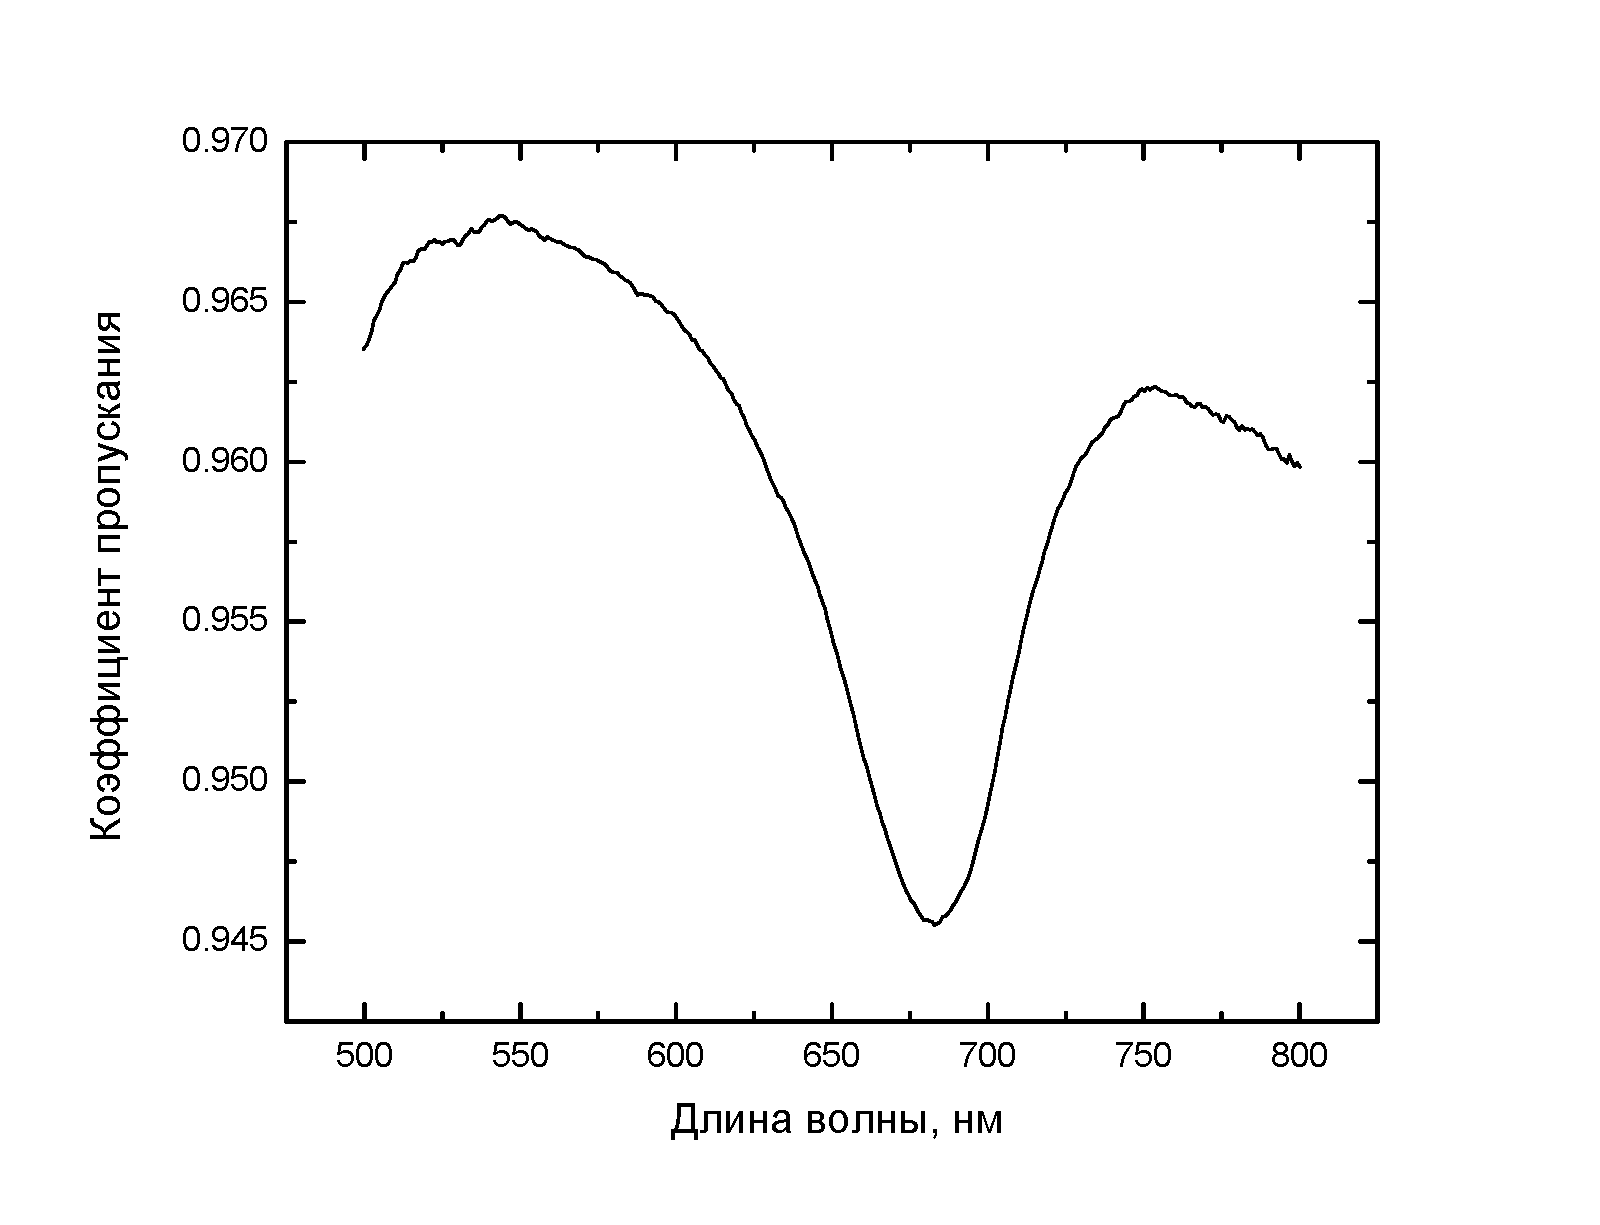
\includegraphics[width=10cm]{img/microspectroscopy/a400d300_spectra.pdf}}
%\caption{Спектр пропускания ансамбля из наностержней с длиной 400 нм и расстоянием 250 нм между ними.}
%\label{img:Spectraa5d3}
%\end{figure}

\begin{figure}
\centering
\begin{subfigure}{.5\textwidth}
  \centering
  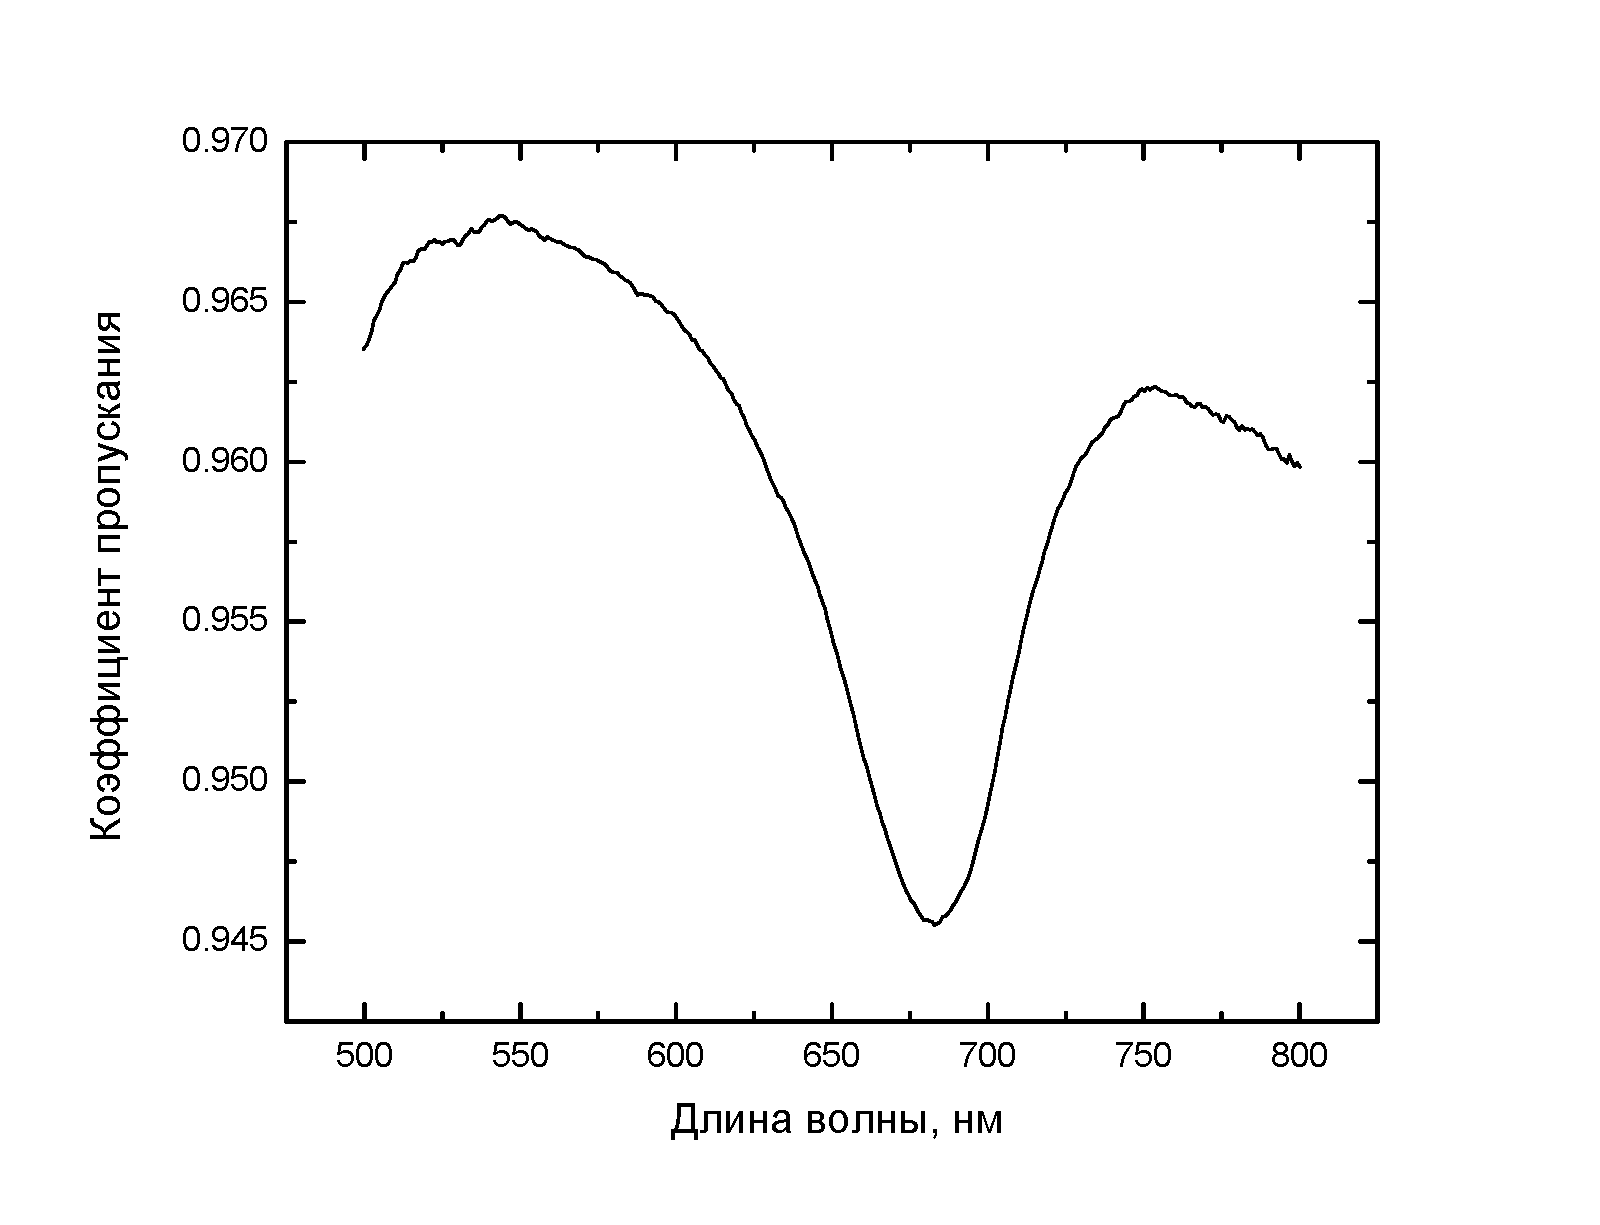
\includegraphics[width=1\linewidth]{img/microspectroscopy/a400d300_spectra.pdf}
  %\caption{График относительного сдвига резонанса второго порядка от расстояния между наностержнями при длине наностержней 500 нм.}
  \label{img:Spectraa5d3}
\end{subfigure}%
\begin{subfigure}{.5\textwidth}
  \centering
  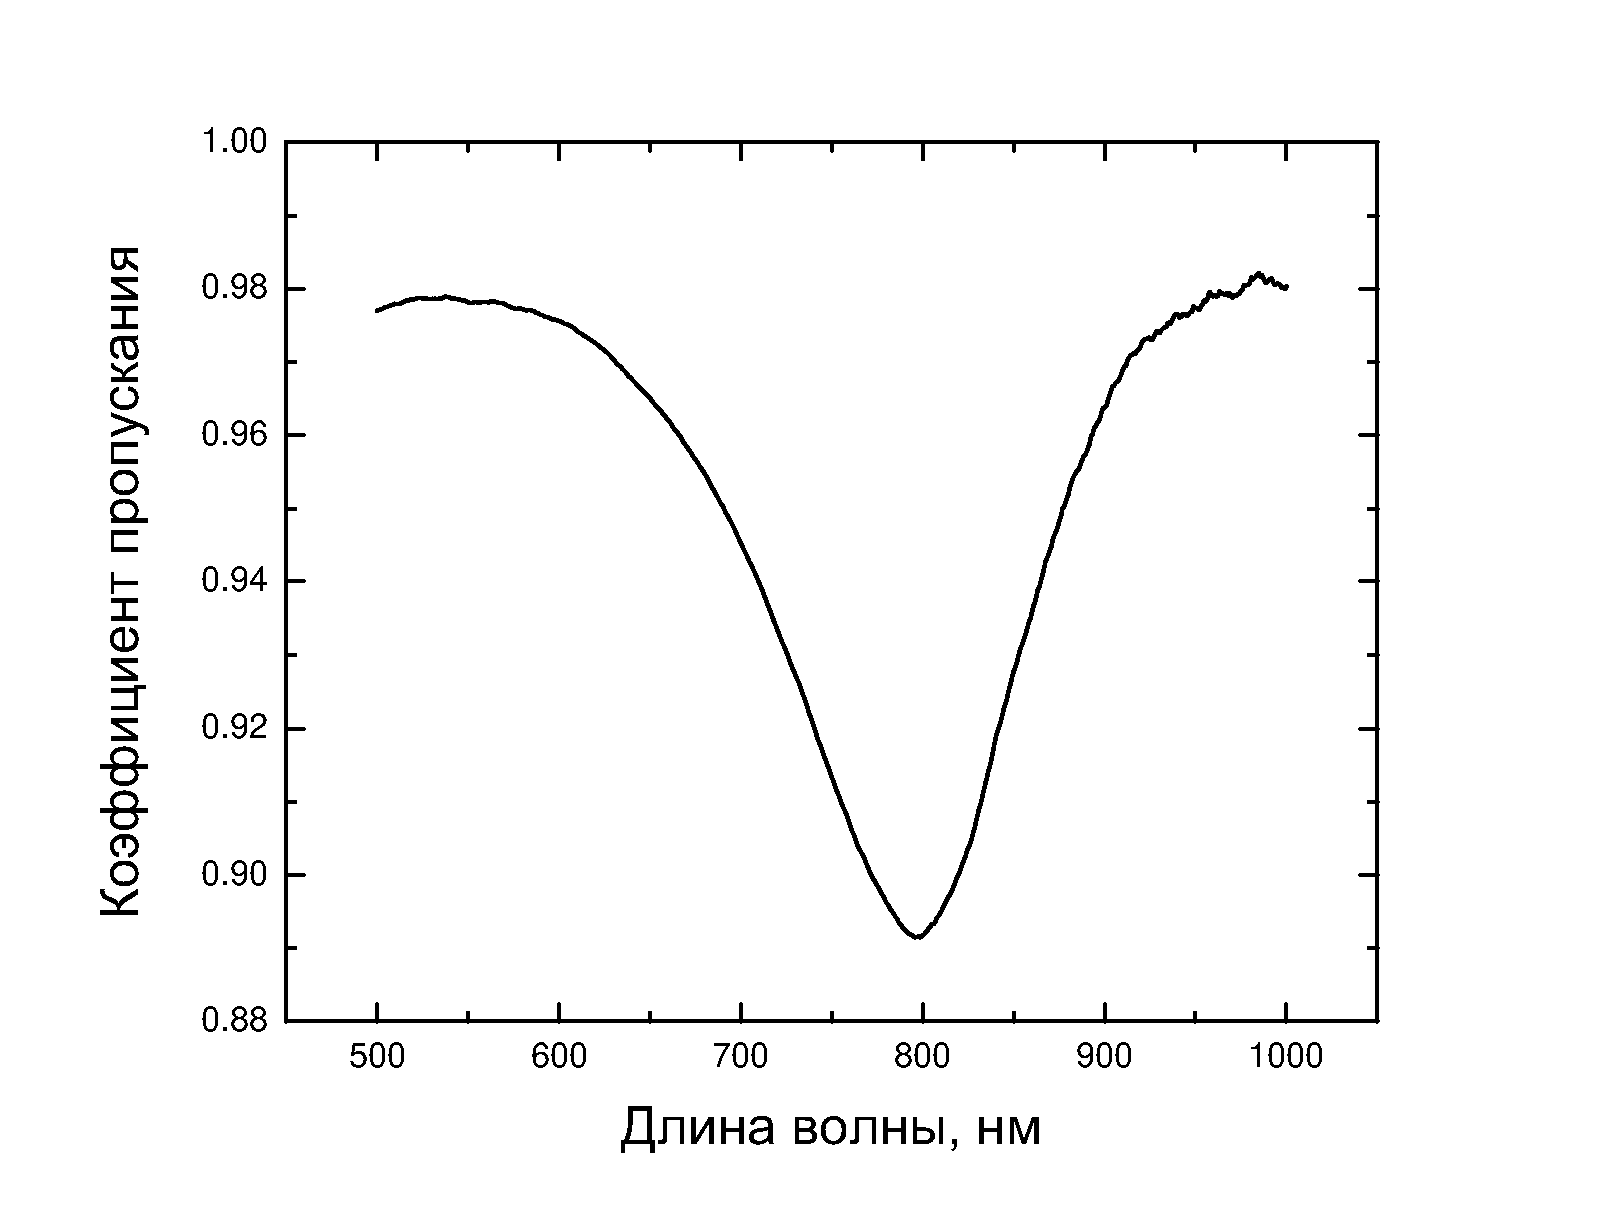
\includegraphics[width=1\linewidth]{img/microspectroscopy/a150d100_spectra.pdf}
  %\caption{График относительного сдвига резонанса второго порядка от расстояния между наностержнями при длине наностержней 400 нм.}
  \label{img:Spectraa1d1}
\end{subfigure}
\caption{Спектр пропускания ансамбля димеров золотых наностержней с длиной  $ a = $ 400 нм и расстоянием $ d = $ 100 нм между ними (слева), $ a = $ 150 нм и $ d = $  100 нм (справа) .}
\label{img:res}
\end{figure}

% BEGIN
\begin{figure}
\center{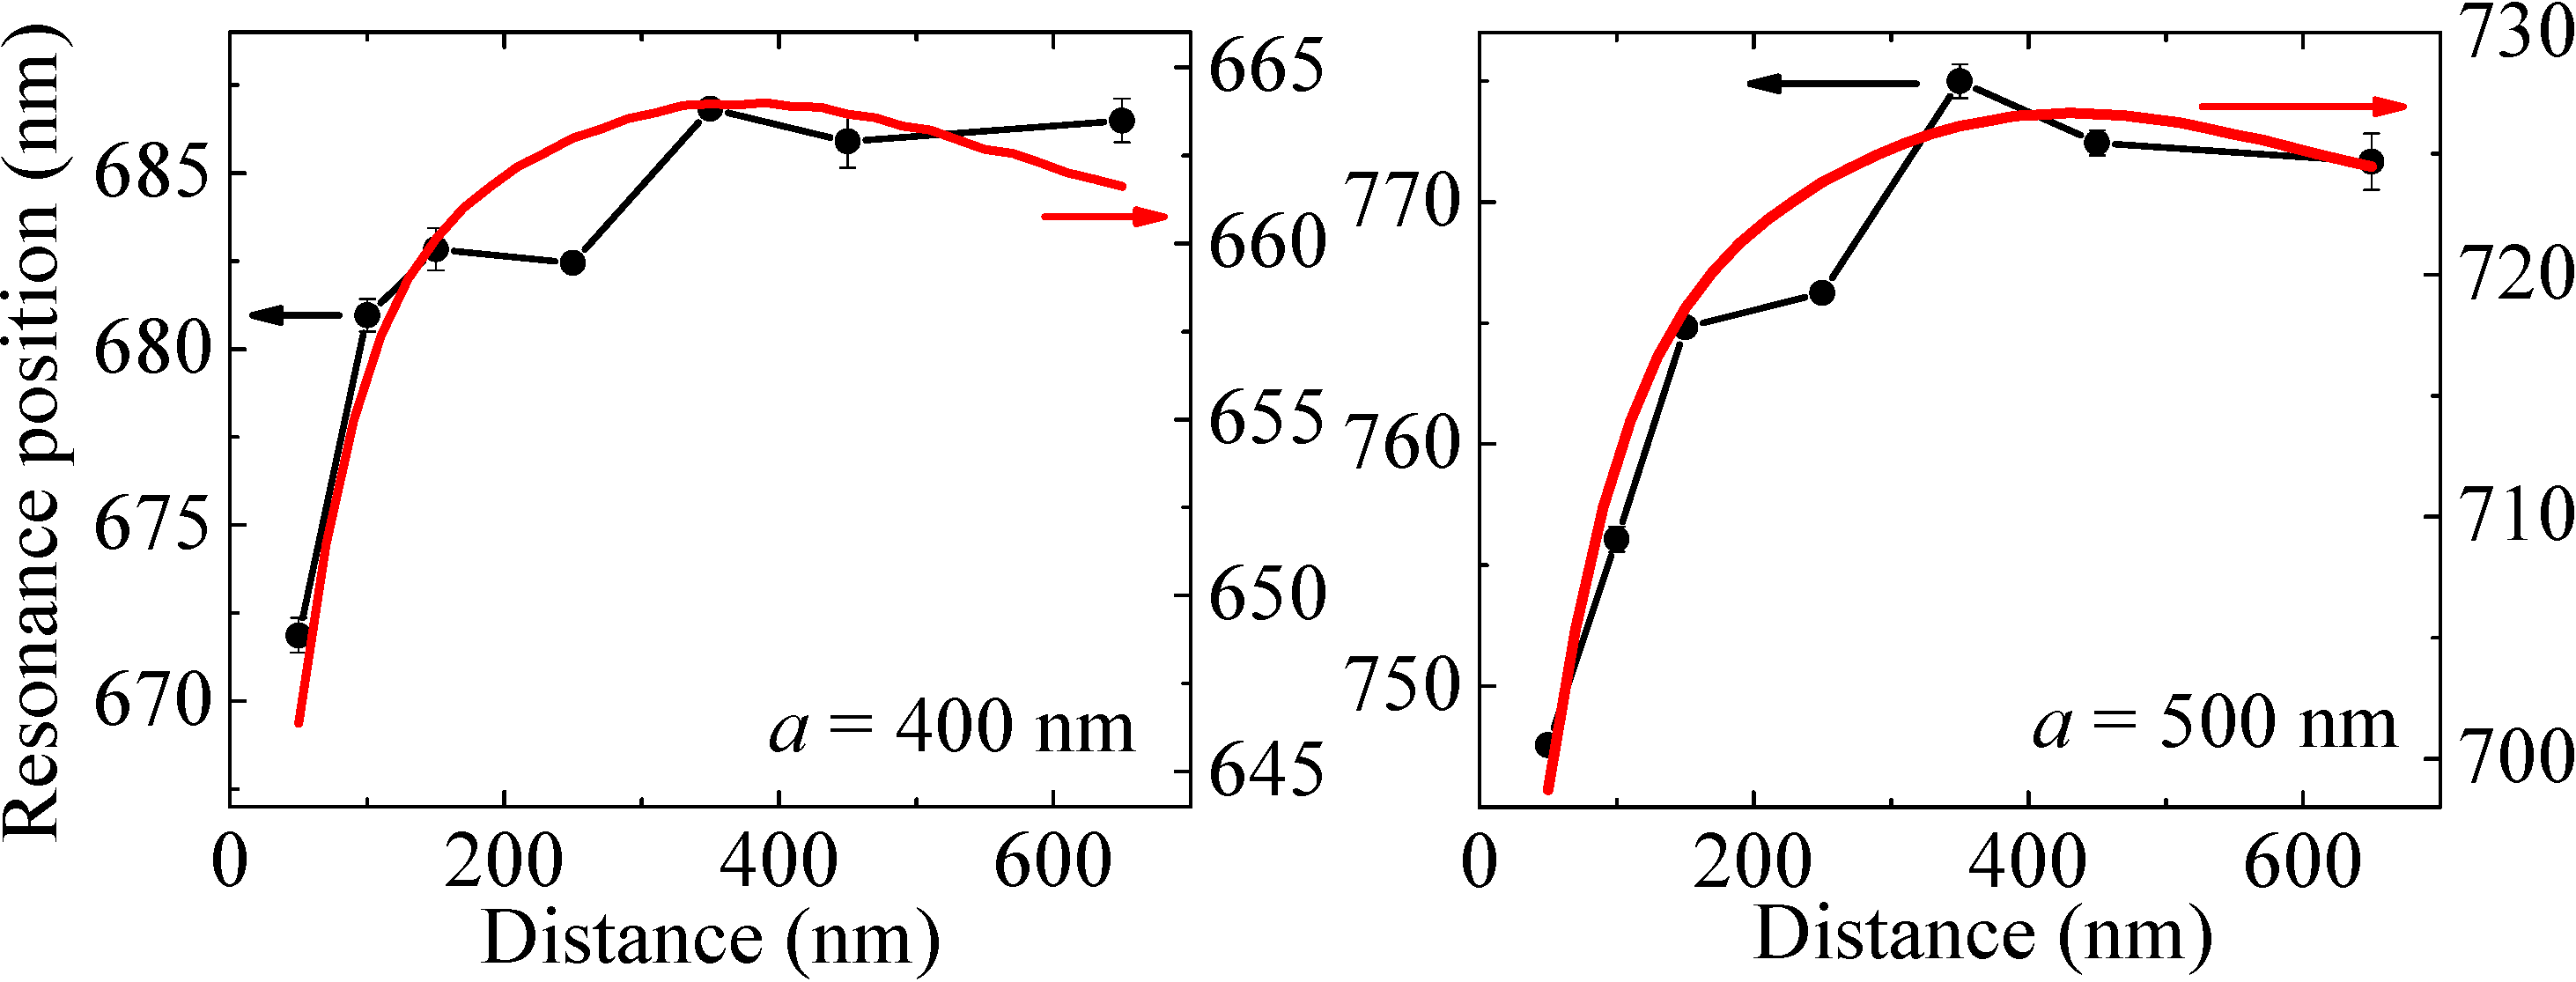
\includegraphics[width=14cm]{img/microspectroscopy/2res_SimExp.pdf}}
\caption{Рассчитанные численно (сплошная линия) и полученные экспериментально (точки) зависимости положения резонанса второго порядка ЛПП от расстояния между наностержнями для длин наностержней $ a = $ 400 нм (a) и $ a = $ 500 нм (b).}
\label{img:2res}
\end{figure}
На рис.~\ref{img:2res} показана зависимость положения резонанса второго порядка как функция расстояния между наностержнями для длин наностержней $ a = $ 400 нм (рис.~\ref{img:2res} a) и $ a = $ 500 нм (рис.~\ref{img:2res} b). Видно, что абсолютные значения положения резонанса различаются в численном расчете и в эксперименте примерно на 100 нм. Это связано с тем, что численном расчете не учитывалась кварцевая подложка, которая влияет на положение резонанса ЛПП. Видно, что абсолютные значения положения резонанса различаются в численном расчете и в эксперименте примерно на 100 нм. Это связано с тем, что численном расчете не учитывалась кварцевая подложка, которая влияет на положение резонанса ЛПП. Также, с уменьшением длины наностержней резонанс ЛПП сдвигается в синюю область. Такое поведение резонанса ЛПП хорошо согласуется с исследованиями систем димеров другой геометрической формы \cite{plasonrulereq, nanoprism}.
% END
%На рис.~\ref{img:a500simexp} показана зависимость положения резонанса второго порядка как функция расстояния между наностержнями для длин наностержней 500 нм, рассчитанная численно (рис.~\ref{img:a500simexp}a) и полученная экспериментально (рис.~\ref{img:a500simexp}б). На экспериментальном графике нанесены систематические ошибки, которые рассчитывались следующим образом. Для фиксированного расстояния между наностержнями в 110 нм рассчитывалось численно положение резонанса второго порядка для длин наностержней 450 нм и 500 нм. Положение резонанса при этом составляло 685 нм и 713 нм. Так как погрешность в длине при изготовлении образцов составляла 3 нм, то систематическая ошибка определения положения резонанса ЛПП  $ \sigma_{err} \approx 2 $ нм. Видно, что абсолютные значения положения резонанса различаются в численном расчете и в эксперименте примерно на 100 нм. Это связано с тем, что численном расчете не учитывалась кварцевая подложка, которая влияет на положение резонанса ЛПП.
%\begin{figure}
%\center{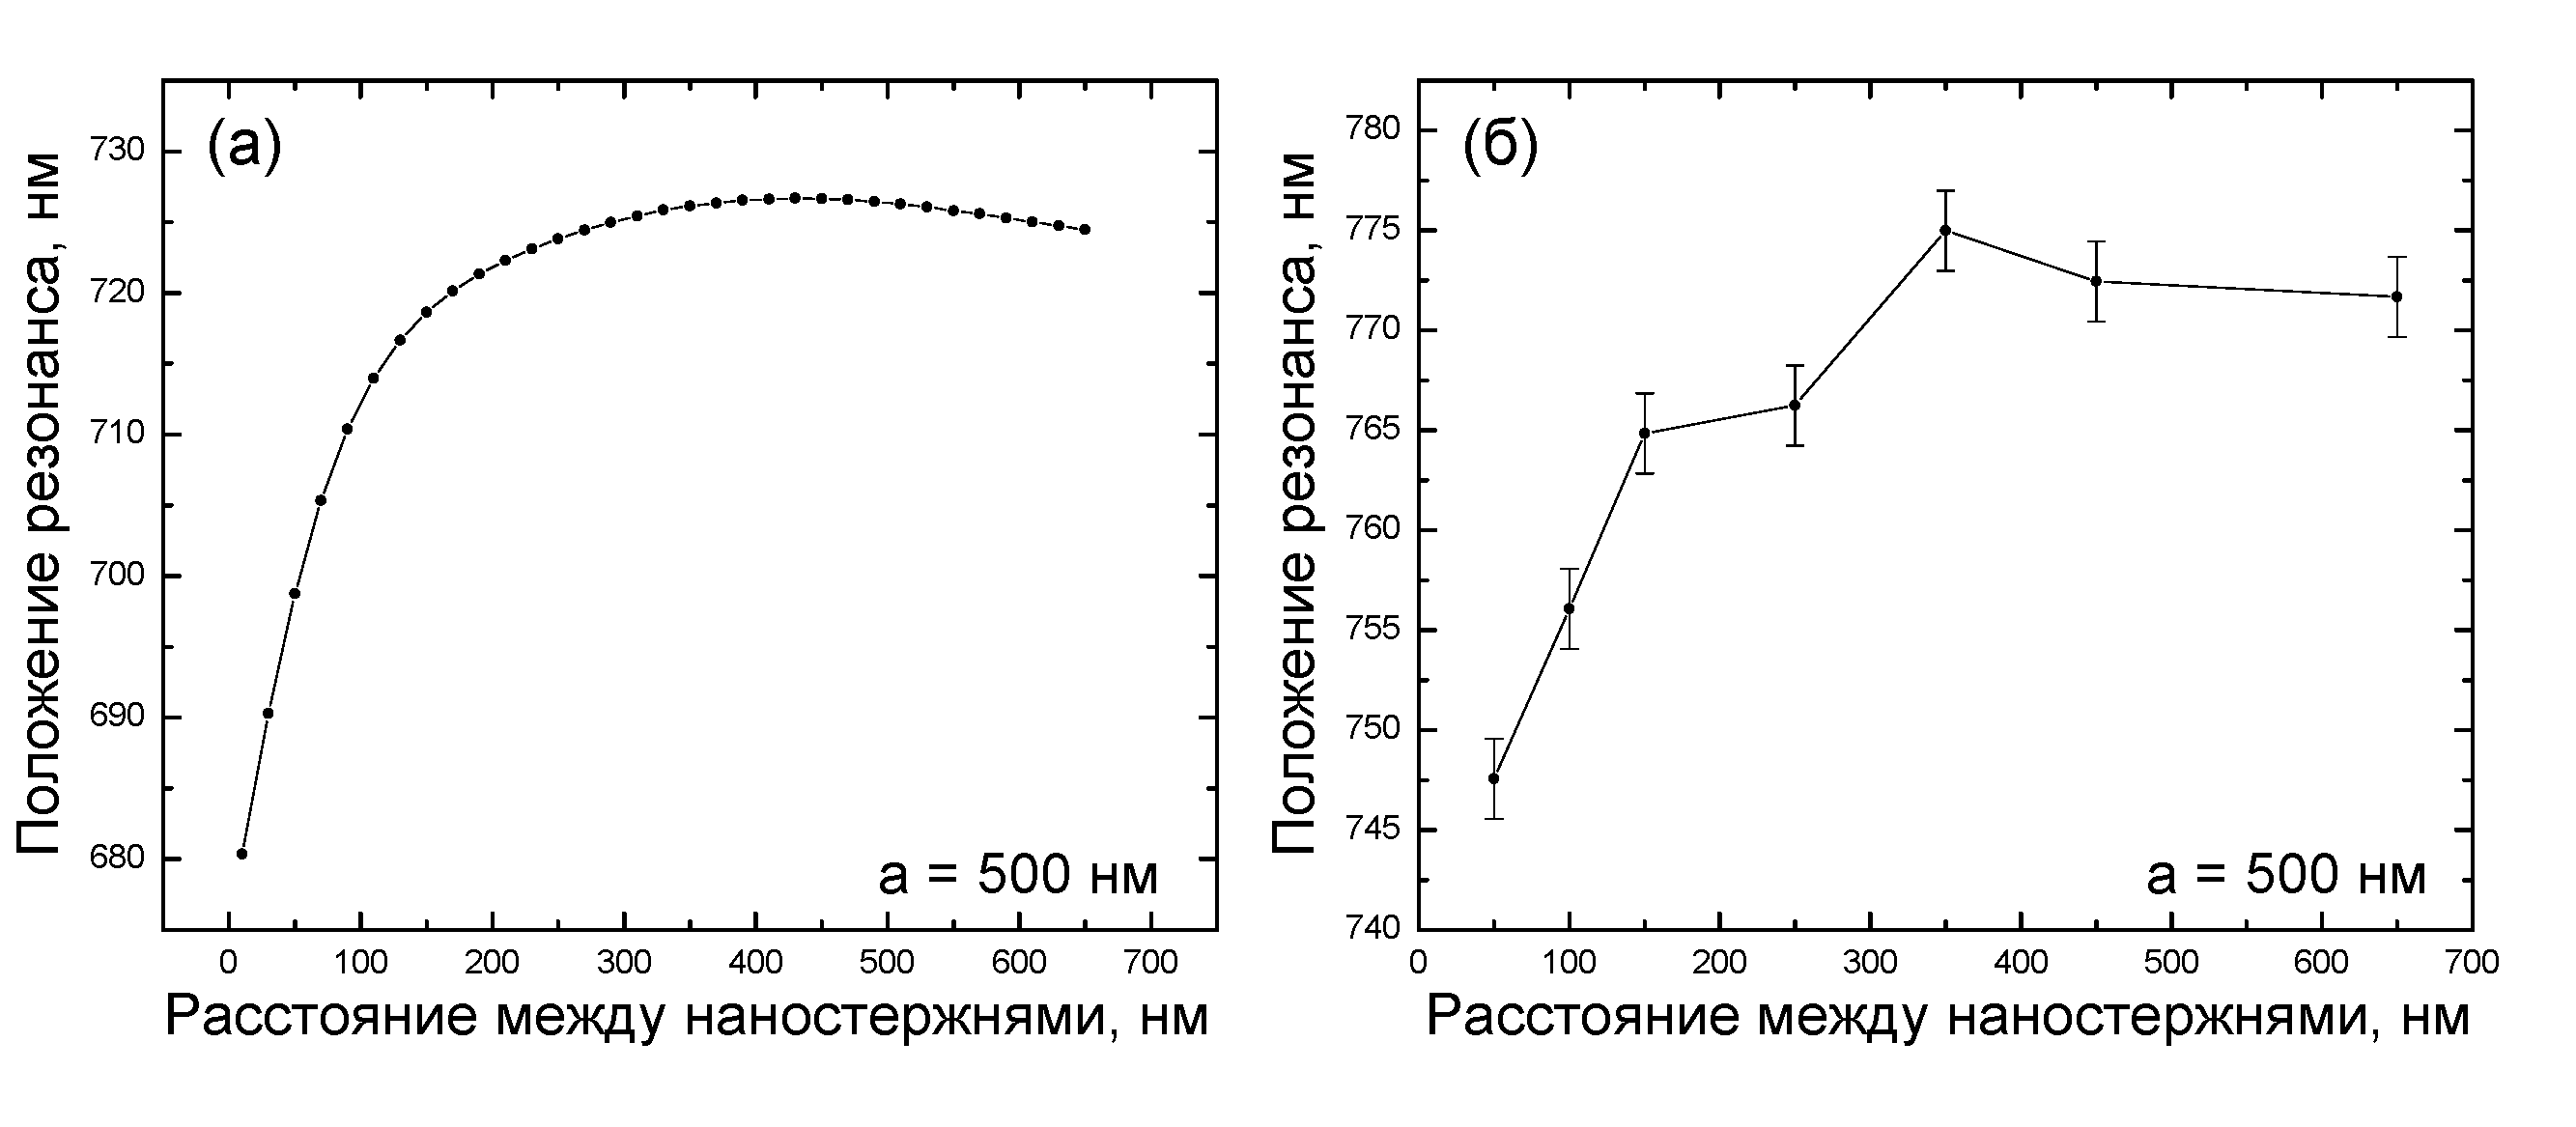
\includegraphics[width=16cm]{img/microspectroscopy/a500simexp.pdf}}
%\caption{Рассчитанный численно (а) и полученный экспериментально (б) график зависимости положения резонанса второго порядка от расстояния между наностержнями для длин наностержней 500 нм. }
%\label{img:a500simexp}
%\end{figure}
%\begin{figure}
%\center{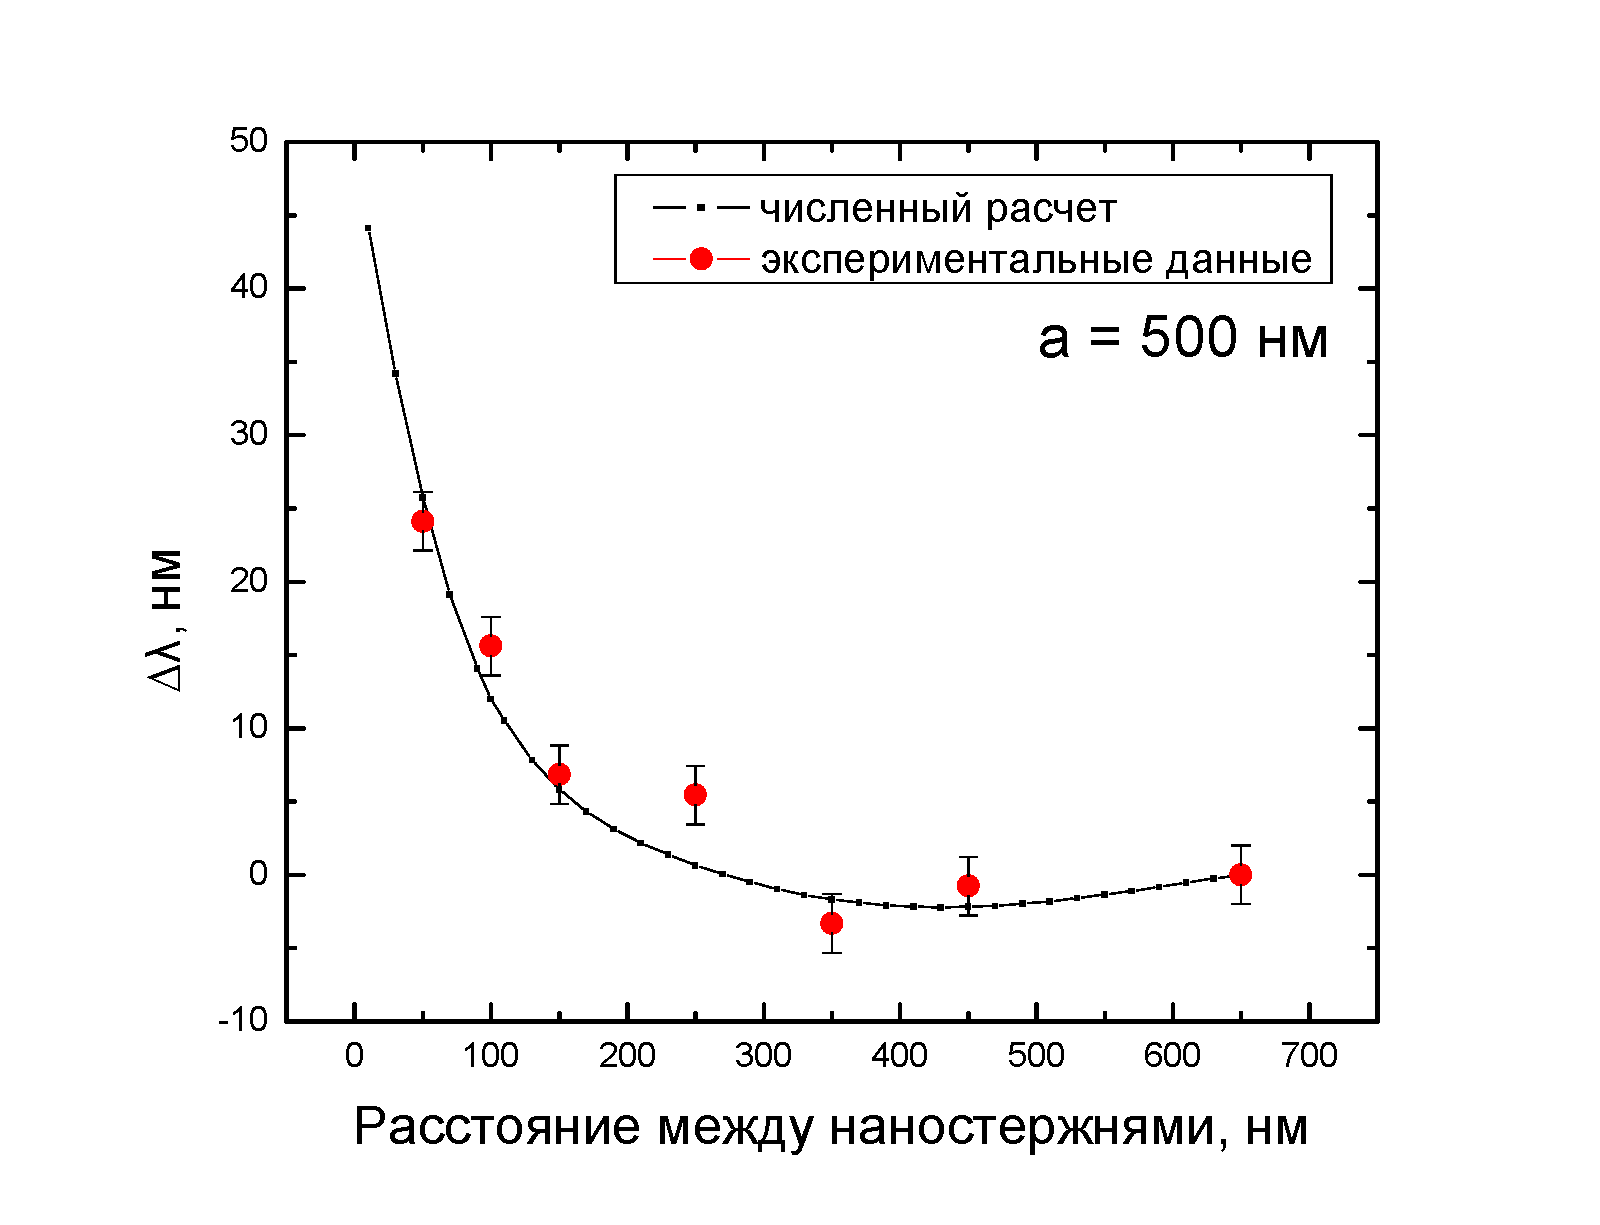
\includegraphics[width=10cm]{img/microspectroscopy/a500shift.pdf}}
%\caption{График относительного сдвига резонанса второго порядка от расстояния между наностержнями при длине наностержней 500 нм.}
%\label{img:a500shift}
%\end{figure}

% Относительный сдвиг 2 в 1
\begin{figure}
\centering
\begin{subfigure}{.5\textwidth}
  \centering
  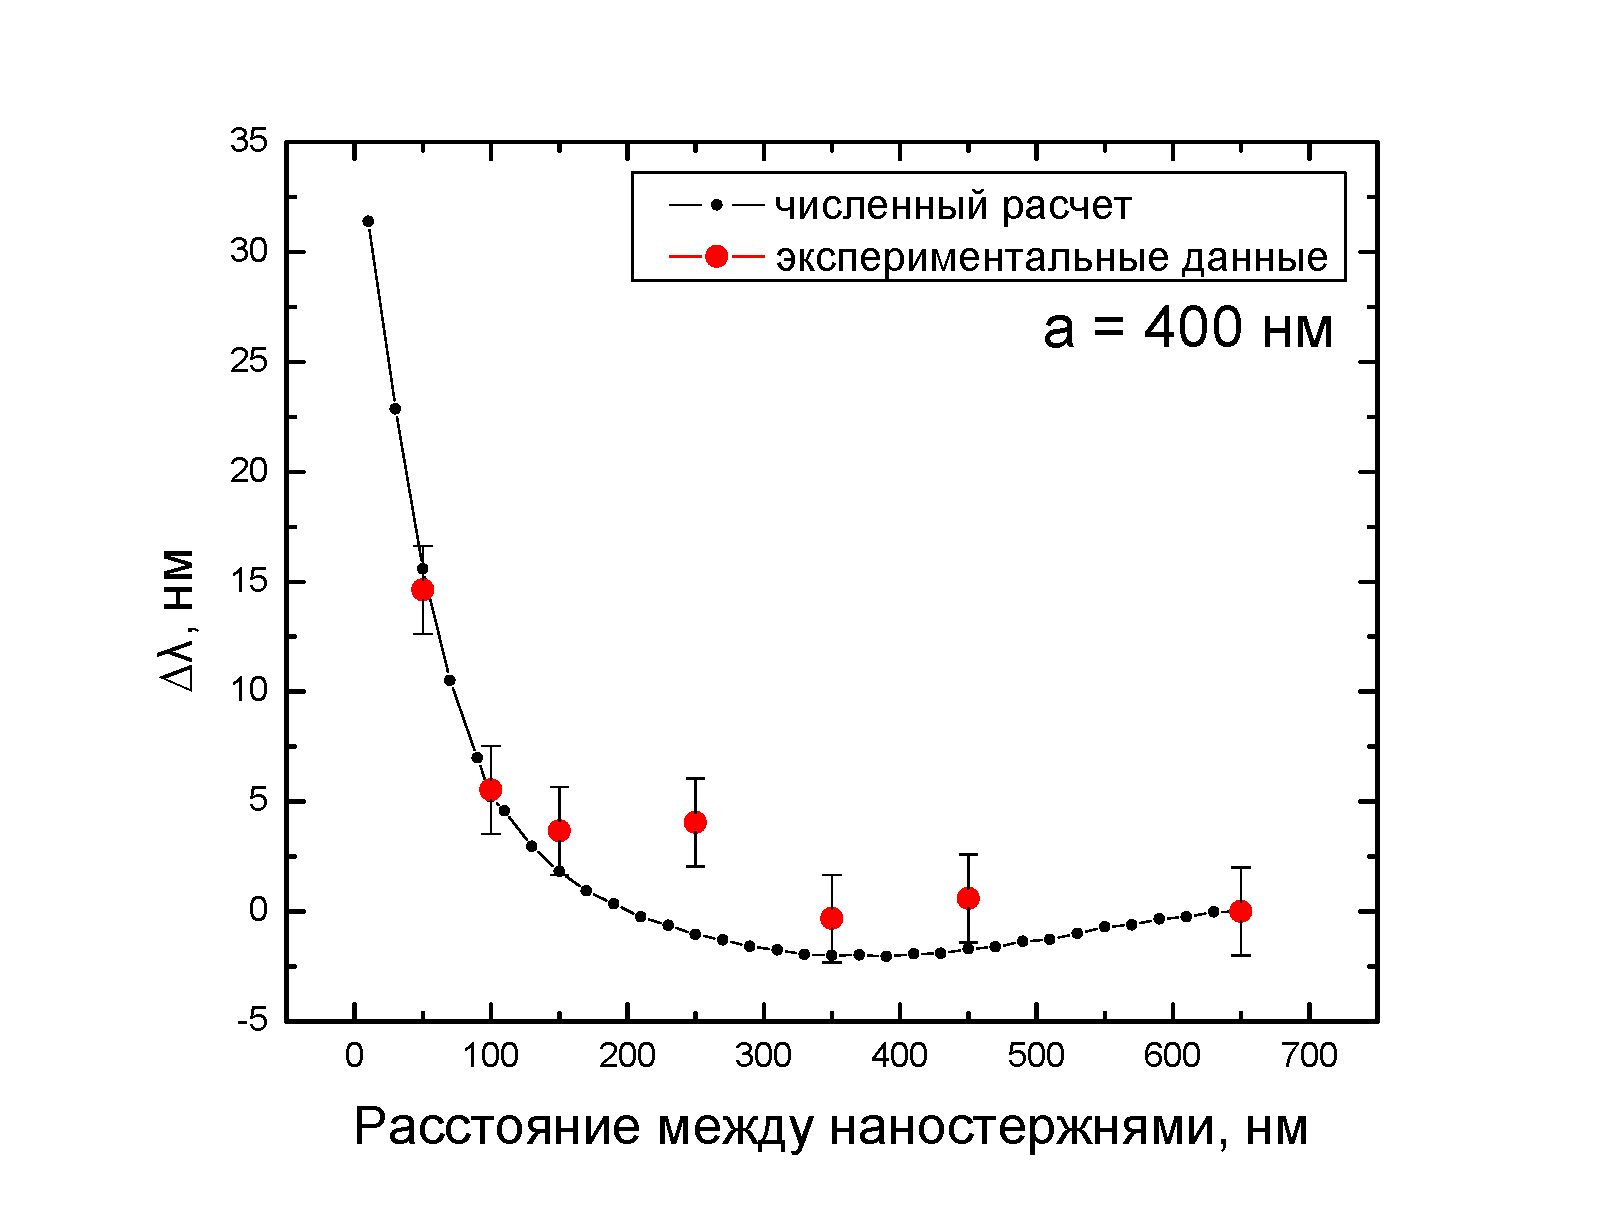
\includegraphics[width=1\linewidth]{img/microspectroscopy/a400shift.pdf}
  %\caption{График относительного сдвига резонанса второго порядка от расстояния между наностержнями при длине наностержней 500 нм.}
  %\label{img:a500shift}
\end{subfigure}%
\begin{subfigure}{.5\textwidth}
  \centering
  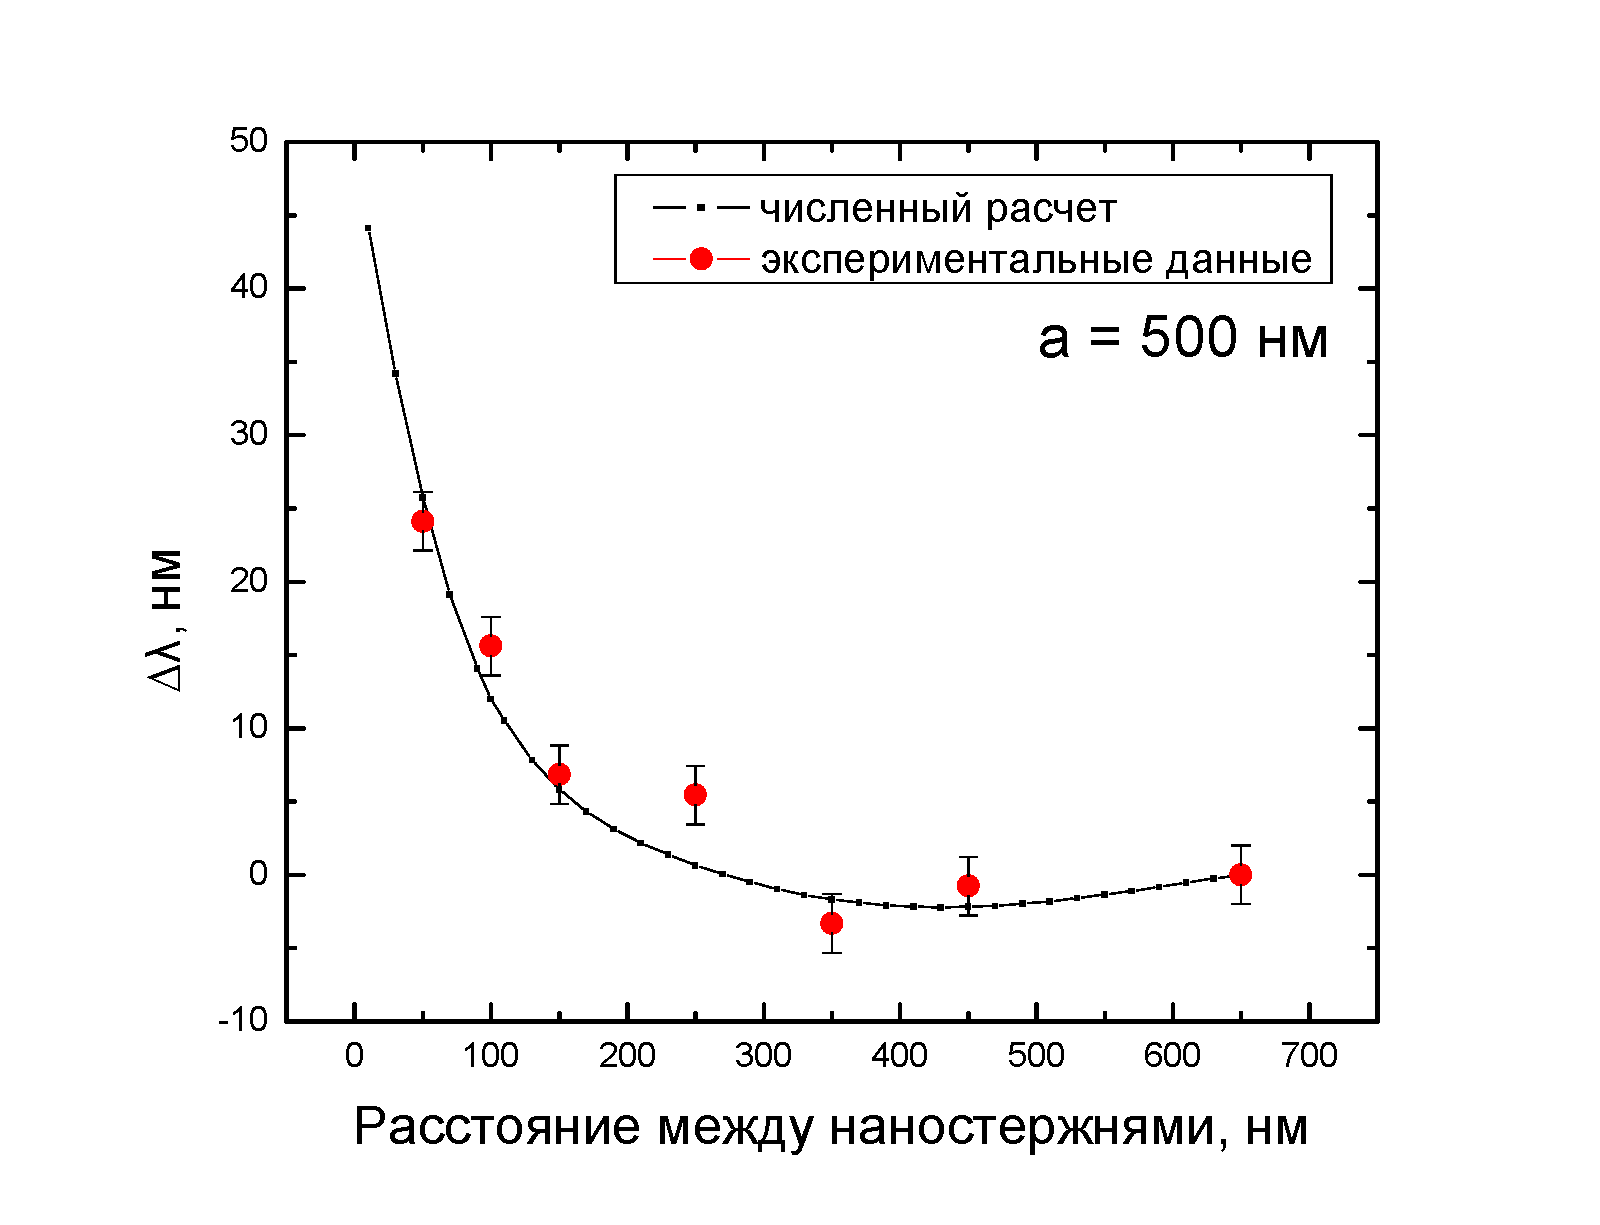
\includegraphics[width=1\linewidth]{img/microspectroscopy/a500shift.pdf}
  %\caption{График относительного сдвига резонанса второго порядка от расстояния между наностержнями при длине наностержней 400 нм.}
  %\label{img:a400shift}
\end{subfigure}
\caption{Графики относительного сдвига резонанса второго порядка от расстояния между наностержнями при длине наностержней $ a = $ 400 нм (слева) и $ a = $ 500 нм (справа).}
\label{img:ashift}
\end{figure}

Графики относительного сдвига резонанса ЛПП второго порядка показаны на рис.~\ref{img:ashift}. Здесь линией обозначены данные численного расчета, а красными точками -- экспериментальные данные. Видно, что численный расчет и экспериментальные данные сходятся в пределах погрешности за исключением точки, в которой расстояние между наностержнями составляет 250 нм. Это может быть связано с дальнепольным дифракционным взаимодействием, которое также влияет на положение резонанса.

Далее исследовался спектр пропускания димеров с длиной 100, 150 и 200 и 300 нм. Характерный спектр пропускания для наностержней длиной 150 нм и расстоянием между наностержнями 100 нм показан на рис.~\ref{img:Spectraa1d1}. Глубина модуляции резонанса ЛПП составляет примерно 10 \%, а ширина на полувысоте резонанса ЛПП --- 100 нм. Для длин наностержней 150 нм данный резонанс является резонансом первого порядка.
На рис.~\ref{img:1res} показана зависимость резонанса первого порядка от расстояния между наностержней для длин наностержней 100, 150, 200 и 300 нм. Зависимость не носит характера насыщения, и наблюдаются осцилляции резонанса ЛПП первого порядка. Это связано, скорее всего, с дальнепольным взаимодействием наностержней, а также дифракционным взаимодействием между димерами, расстояние между которыми $ \approx 1$ мкм. Данные осцилляции являются паразитными для задачи построения <<плазмонной линейки>>, поскольку они мешают построению калибровочной кривой. Таким образом из экспериментальных данных следует, что для резонанса второго порядка возможно построить <<плазмонную линейку>> из-за его слабой чувствительности к дальнепольному взаимодействию, а для резонанса первого порядка влияние дальнопольного взаимодействия приводят к невозможности построения <<плазмонной линейки>>.
\begin{figure}
\center{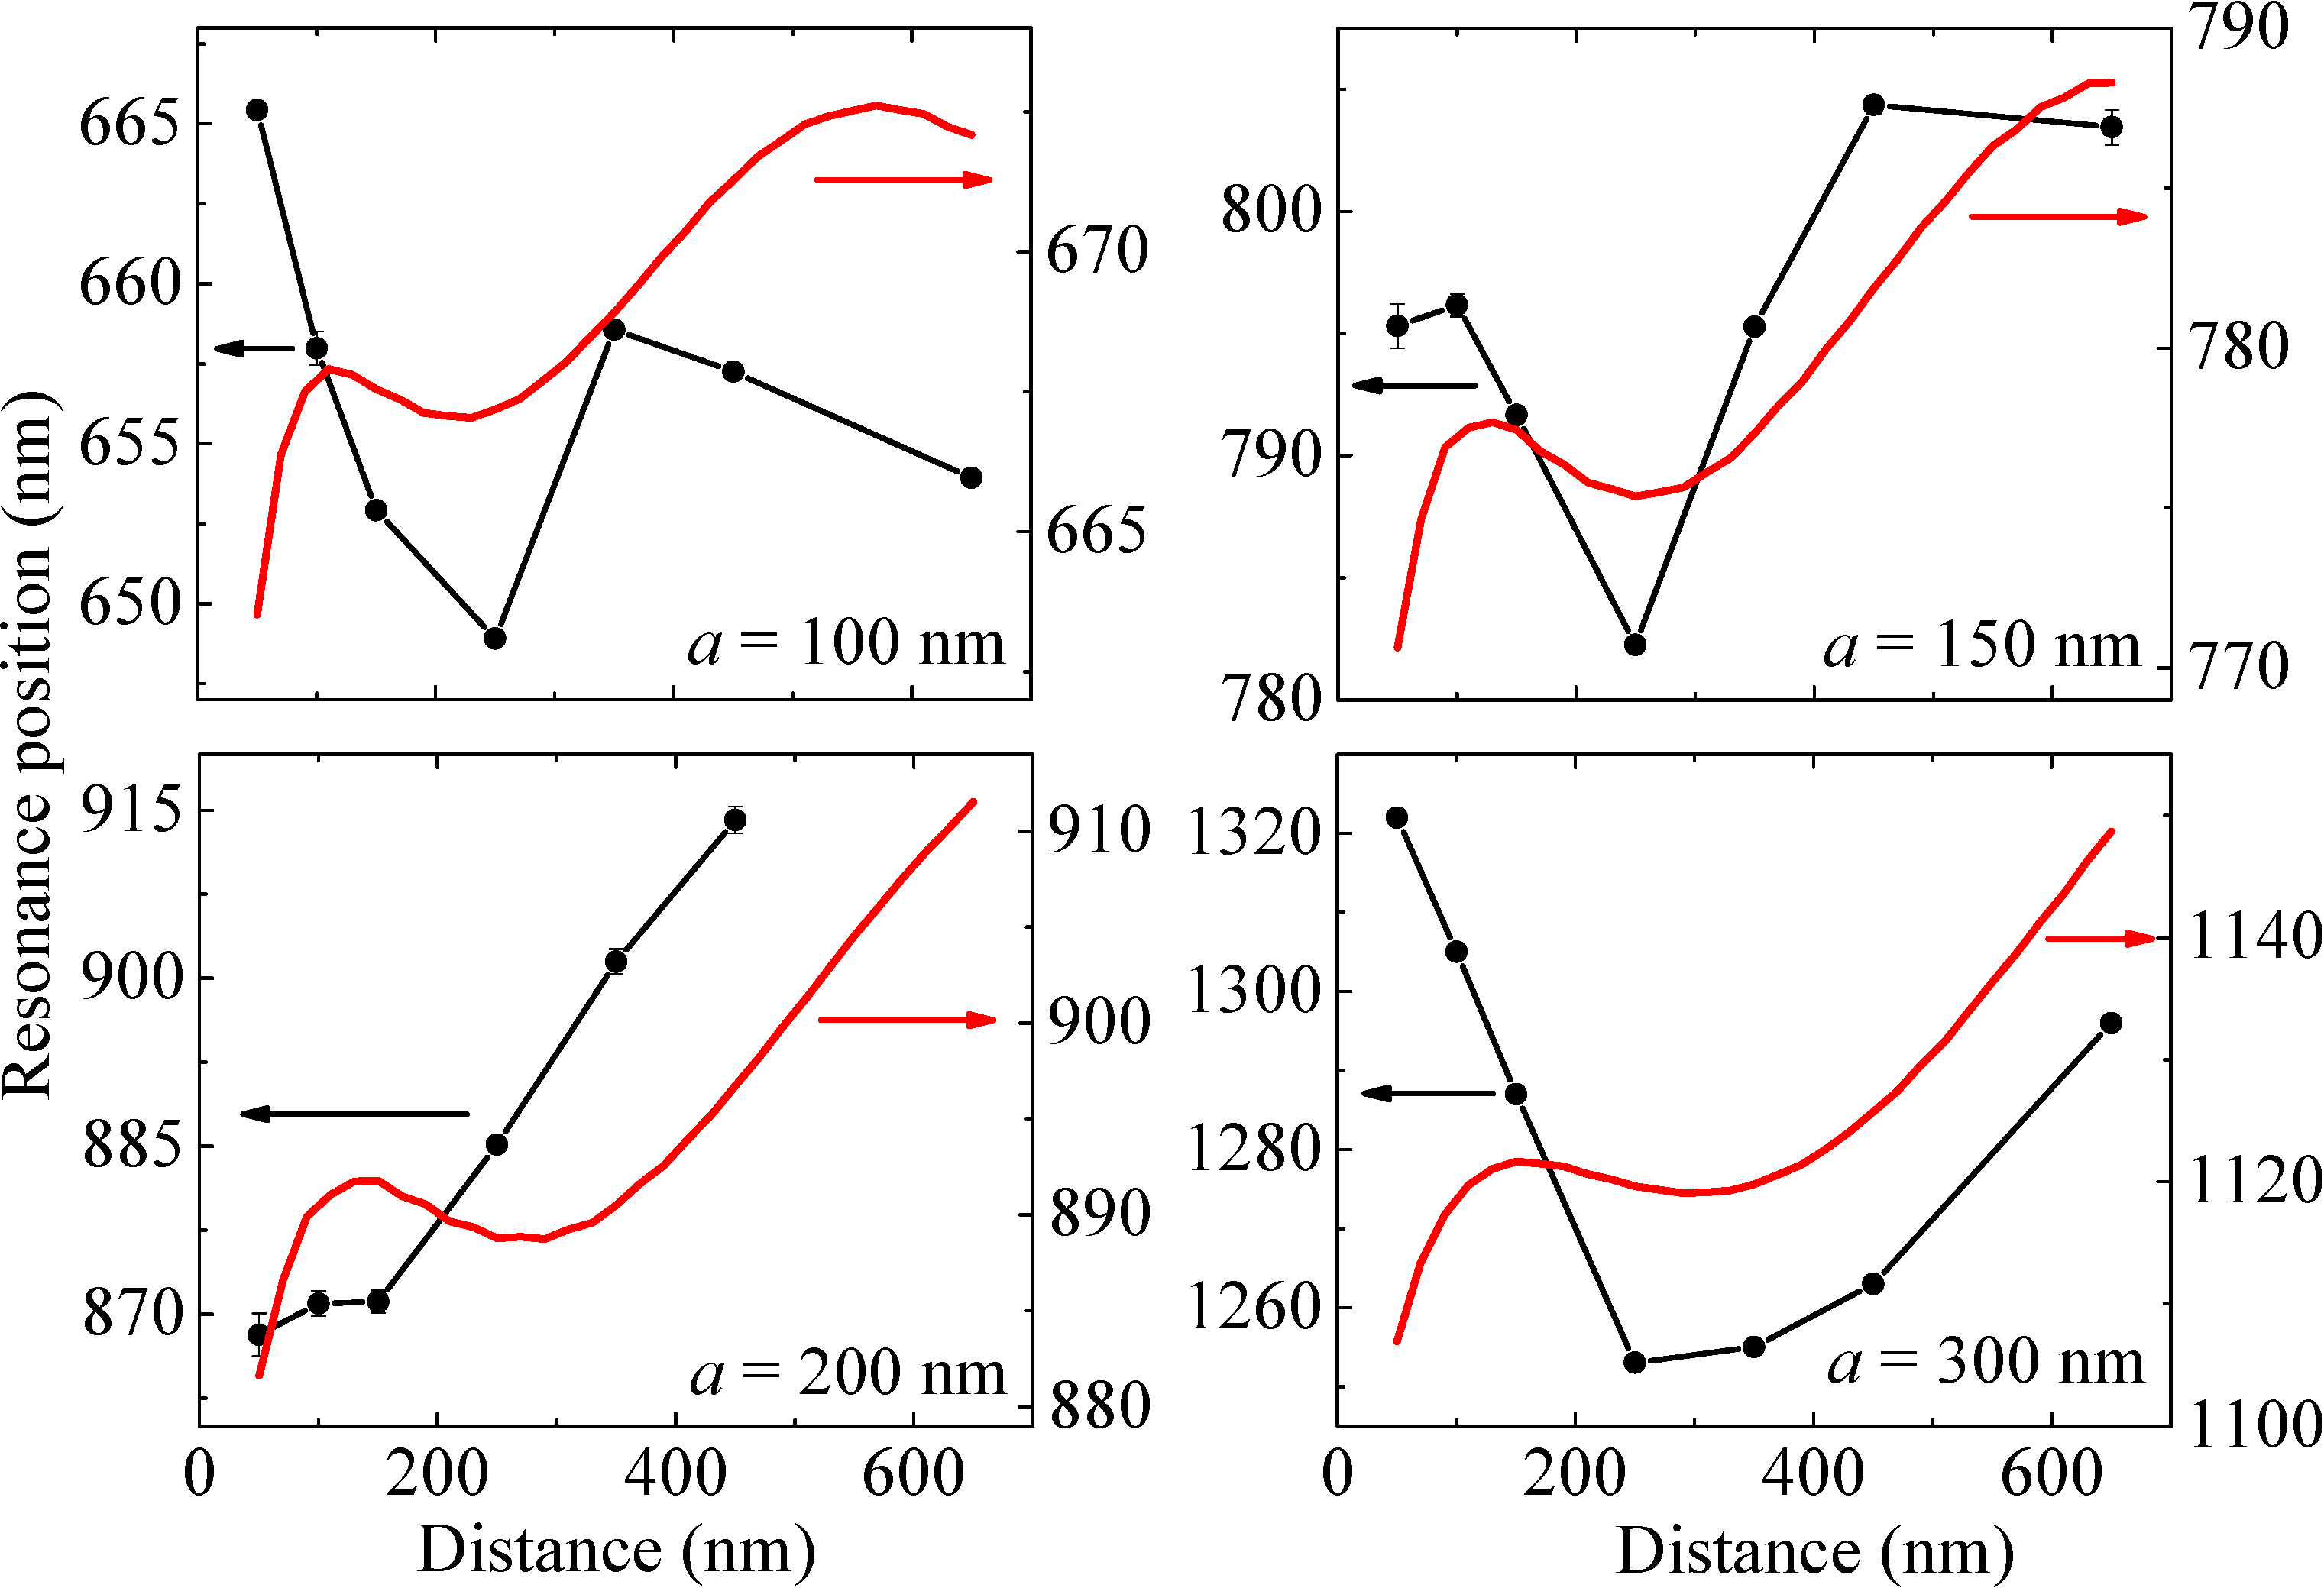
\includegraphics[width=1.0\linewidth]{img/microspectroscopy/1res.pdf}}
\caption{Рассчитанные численно (сплошная линия) и полученные экспериментально (точки) зависимости положения резонанса первого порядка ЛПП от расстояния между наностержнями для длин наностержней $ a = $ 100, 150, 200 и 300 нм.}
\label{img:1res}
\end{figure}

